\documentclass{beamer}
\usepackage[english,russian]{babel}
\usepackage[utf8]{inputenc}
\usepackage{pagenumber}

\usepackage{hyperref}
% Стиль презентации
\usetheme[numbers, totalnumbers]{Dresden}
% цветовая схема
\usecolortheme{beaver}

\makeatletter
\defbeamertemplate*{footline}{Dresden}{
	\leavevmode%
	\hbox{%
	\begin{beamercolorbox}[wd=.15\paperwidth,ht=2.25ex,dp=1ex,center]{author in head/foot}%
		\usebeamerfont{author in head/foot}%
		\insertauthor	
	\end{beamercolorbox}%
	\begin{beamercolorbox}[wd=0.7\paperwidth,ht=2.25ex,dp=1ex,center]{title in head/foot}%
		\usebeamerfont{title in head/foot}\inserttitle
	\end{beamercolorbox}%
	\begin{beamercolorbox}[wd=.15\paperwidth,ht=2.25ex,dp=1ex,right]{date in head/foot}%
		\usebeamerfont{date in head/foot}\hspace*{2em}
		\insertframenumber{} / \inserttotalframenumber\hspace*{2ex}
	\end{beamercolorbox}}%
}
\makeatother

\begin{document}
\title{Пространственно-кинематическое моделирование подсистем Галактики}  
\author{Волков Д.В.}
\institute{научный руководитель Никифоров И.И. \\ Санкт-Петербургский государственный университет }
\date{кафедра небесной механики и звездной астрономии, \\ \today} 
% Создание заглавной страницы
\frame{\titlepage} 

\begin{frame}{О каталоге}
	\begin{itemize}
		\item 29502 объекта.
		\item Очень точные данные о лучевых скоростях.	
                \item Имеются данные для собственных движений для большинства объектов (UCAC-4 & HSOY)
		\item Точность измерения гелиоцентрических расстояний.
		\item Каталог обновляется.
	\end{itemize}
\end{frame}

\begin{frame}{О каталоге}
	\begin{center}
	\begin{figure}[h]
\begin{minipage}[h]{0.8\linewidth}
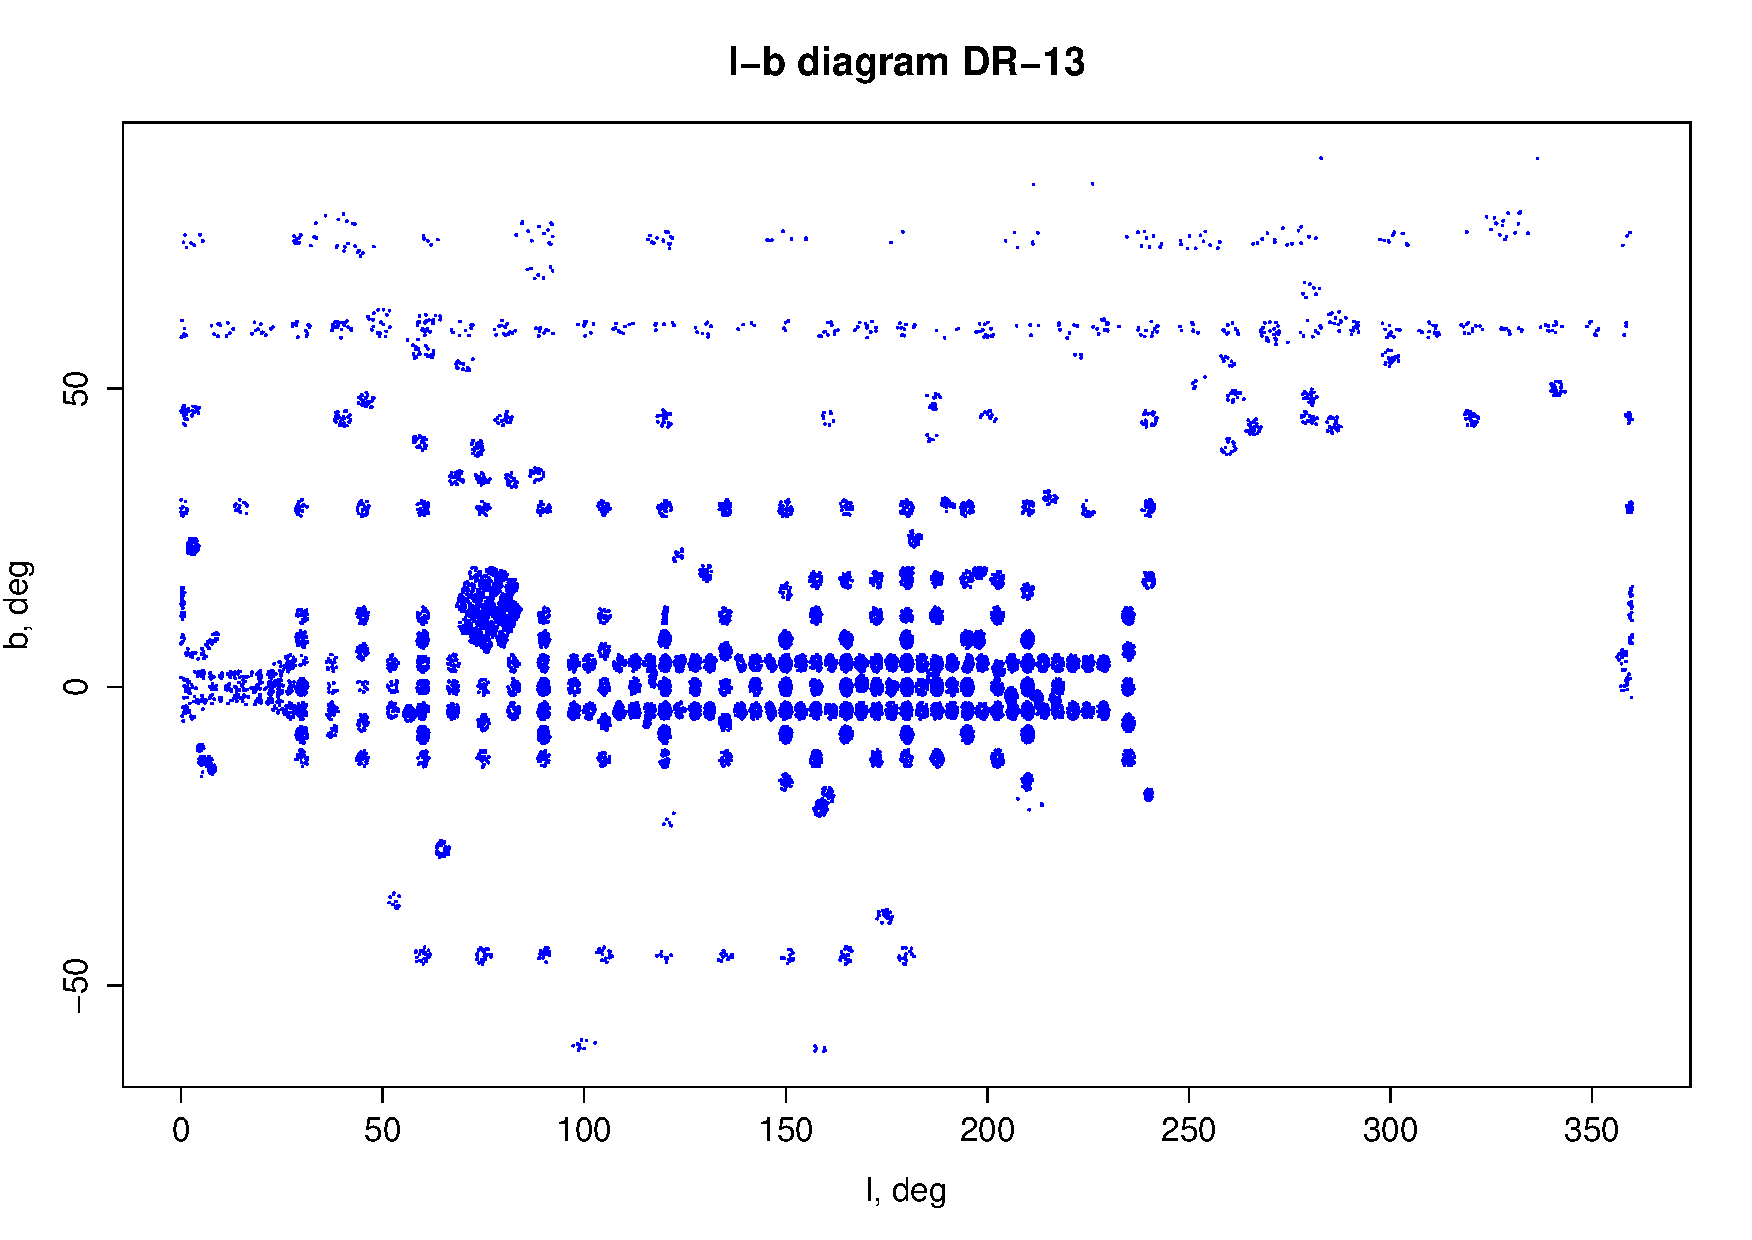
\includegraphics[width=1\linewidth]{pdf/lb_dr13.pdf}
\end{minipage}
\end{figure}
	\end{center}
\end{frame}

\begin{frame}{О каталоге}
	\begin{center}
	\begin{figure}[h]
\begin{minipage}[h]{0.8\linewidth}
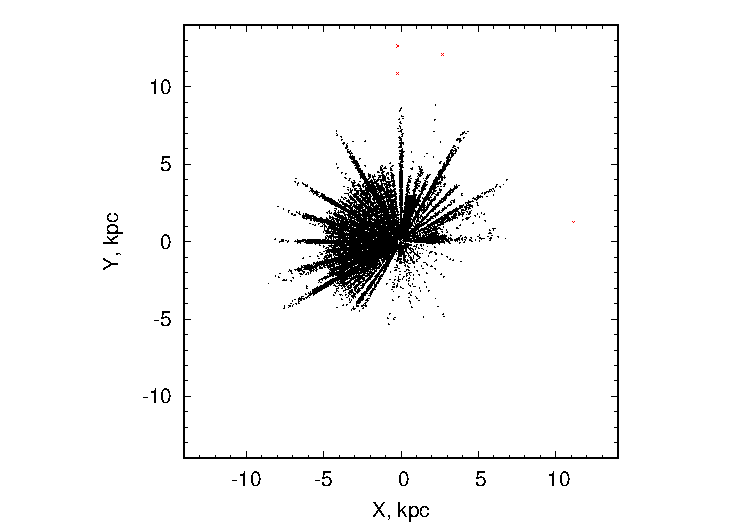
\includegraphics[width=1\linewidth]{pdf/xy.pdf}
\end{minipage}
\end{figure}
	\end{center}
\end{frame}

\begin{frame}{О каталоге}
	\begin{center}
	\begin{figure}[h]
\begin{minipage}[h]{0.8\linewidth}
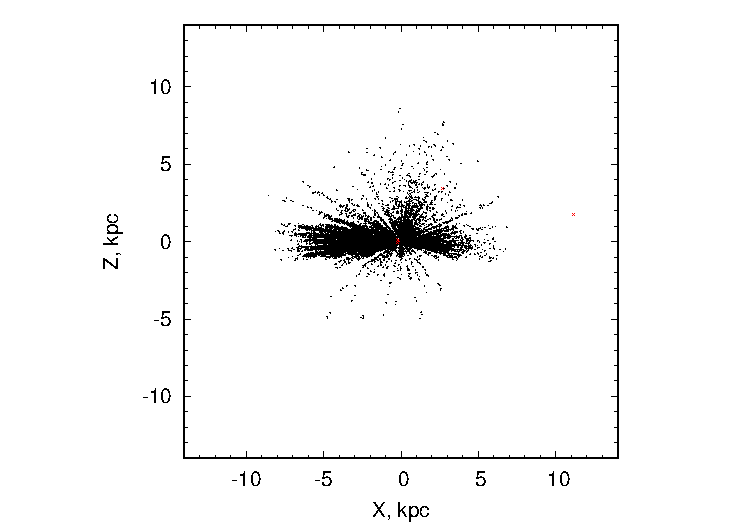
\includegraphics[width=1\linewidth]{pdf/xz.pdf}
\end{minipage}
\end{figure}
	\end{center}
\end{frame}

\begin{frame}{О каталоге}
	\begin{center}
	\begin{figure}[h]
\begin{minipage}[h]{0.8\linewidth}
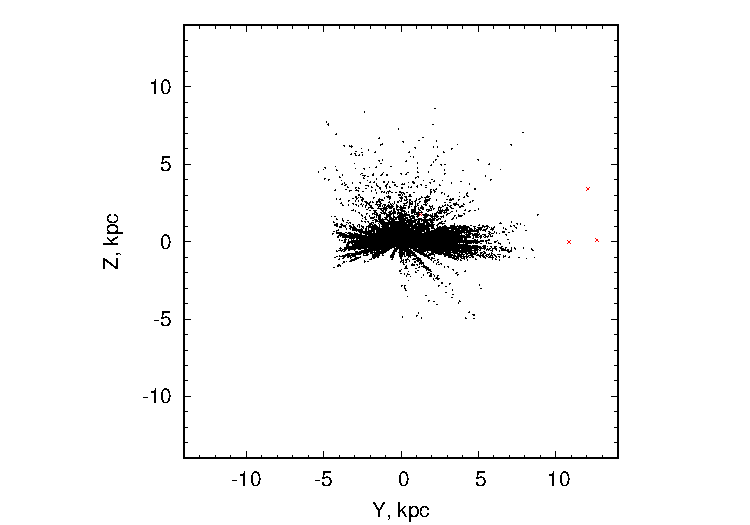
\includegraphics[width=1\linewidth]{pdf/yz.pdf}
\end{minipage}
\end{figure}
	\end{center}
\end{frame}

\begin{frame}{Модельные предположения}
	\begin{itemize}
		\item Линейная скорость $\theta$ движения подсистем Галактики -- функция от $R$:$$\theta = \theta (R) $$ 
			(цилиндрический закон вращения), т.е. исследуемая подсистема плоская.
	\end{itemize}
\end{frame}

\begin{frame}{Обозначения}
	\begin{equation}
		V_{r, \texttt{mod}} = V_{r, \texttt{rot}} + V_{r, \odot},
	\end{equation}
	
	\begin{equation}
		V_{r, \texttt{rot}} = (\omega - \omega_0)R_0 \sin{l} \cos{b},
	\end{equation}
		
	\begin{equation}
		V_{r, \odot} = -u_{\odot} \cos{l} \cos{b} - v_{\odot} \sin{l} \cos{b} - w_{\odot} \sin{b}.
	\end{equation}
\end{frame}

\begin{frame}{Уравнения кинематической модели}
	\begin{equation}
		\Theta_n(R) = \sum^n_{k = 0} \frac{\theta_k}{k!} \left( \Delta R \right)^k.
	\end{equation}
\begin{equation}
\Delta R = R - R_0,
\end{equation}
\begin{equation}
	R = \sqrt{R_0^2 + r^2 \cos^2{b} - 2R_0 r \cos{l} \cos{b}}.
\end{equation}

%\end{frame}

%\begin{frame}{Уравнения кинематической модели}
	Для $V_r$ общий вид модели:
	\begin{equation}
		V_{r, \texttt{mod}} = \left[ -2A\Delta R + \sum^n_{k = 2} \frac{\theta_k}{k!} \left( \Delta R \right)^k \right] \frac{R_0}{R} \sin{l} \cos{b} + V_{r, \odot},
	\end{equation}
	\begin{equation}
		A = - \frac{1}{2} R_0 \omega^{'}(R_0) = - \frac{1}{2} (\theta_1 - \omega_0).
	\end{equation}
\end{frame}

\begin{frame}{Решение}
	Решается система уравнений
	\begin{equation}
		V_r = V_{r, \texttt{mod}} (R_0, A, \theta_2, \:\ldots,\: \theta_n, u_{\odot}, v_{\odot}, w_{\odot}).
	\end{equation}
	Оценка дисперсии
	\begin{equation}
		\sigma^2_{V_r} = \frac{1}{N - n - 4} \sum^N_{i = 1} \left( V_r - V_{r, \texttt{mod}} \right)^2_i.
	\end{equation}
\end{frame}

\begin{frame}{Решение для модели с $V_r$}
\begin{itemize}
\item Выбор оптимального порядка полинома,
\item Исключение пространственно и/или кинематически изолированых объектов.
\item Исключение объектов по избыточным невязкам (Никифоров, 2012).
\end{itemize}
\end{frame}

\begin{frame}{Выбор оптимального порядка полинoма}
	Критерии:
	\begin{itemize}
		\item Значимость старших коэффициентов,
		\item Зависимость дисперсии от порядка,
		\item Вид кривой вращения для данного порядка.
	\end{itemize}
\end{frame}

\begin{frame}{Зависимость дисперсии от порядка}
\begin{figure}[h]
\begin{minipage}[h]{0.8\linewidth}
	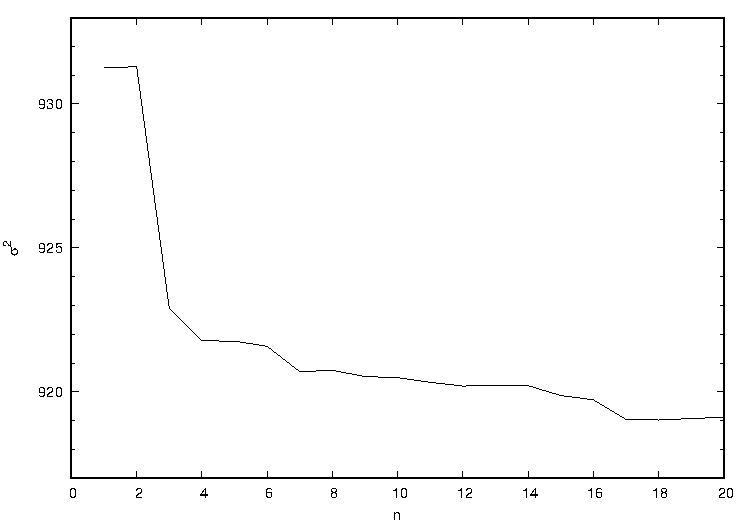
\includegraphics[width=1\linewidth]{pdf/sigmas.pdf}
\end{minipage}
\end{figure}
\end{frame}

\begin{frame}{Исключение по невязкам}
	\begin{itemize}
		\item Для данной мощности выборки вычисляется значение $\kappa$
			\begin{equation}
				\big(1 - \psi(\kappa)\big) N = 1,
			\end{equation}
			где $\psi(\kappa)$ -- интеграл
			\begin{equation}
				\psi(\kappa) = \sqrt{\frac{2}{\pi}} \int^{\kappa}_{0} e^{-\frac{1}{2}t^2} dt.
			\end{equation}
		\item Исключаются объекты с невязками
			\begin{equation}
				\frac{| \varepsilon_i |}{\sigma_i} > \kappa
			\end{equation}
	\end{itemize}
	\begin{center}
\end{center}
\end{frame}

\begin{frame}{Уравнения кинематической модели}
Для собственных движений $\mu_b = \frac{db}{dt}$:
	\begin{equation}
		k\mu_{b, \texttt{mod}} = k\mu_{b, \texttt{rot}} + k\mu_{b, \odot},
	\end{equation}
	\begin{equation}
		k\mu_{b, \texttt{mod}} = \left[ 2A\Delta R - \sum^n_{k = 2} \frac{\theta_k}{k!} \left( \Delta R \right)^k \right] \frac{R_0}{Rr} \sin{l} \sin{b},
	\end{equation}
	\begin{equation}
                k\mu_{b, \odot} = \frac{u_{\odot}\cos{l}\sin{b} + v_{\odot}\sin{l}\sin{b} - w_{\odot}\cos{b}}{r}.
	\end{equation}
        Здесь и далее полагаем $k=4.7406$.
\end{frame}

\begin{frame}{Уравнения кинематической модели}
Для собственных движений $\mu_l = \frac{dl}{dt}$:
	\begin{equation}
		k\mu_{l, \texttt{mod}} = k\mu_{l, \texttt{rot}} + k\mu_{l, \odot},
	\end{equation}
	\begin{equation}
                k\mu_{l, \texttt{mod}} = \left[ -2A\Delta R + \sum^n_{k = 2} \frac{\theta_k}{k!} \left( \Delta R \right)^k \right] \left( \frac{R_0\cos{l}}{r} - \cos{b} \right) R^{-1} - \omega_0 \cos{b},
	\end{equation}
	\begin{equation}
                k\mu_{b, \odot} = \frac{u_{\odot}\sin{l}- v_{\odot}\cos{l}}{r}.
	\end{equation}
\end{frame}

\begin{frame}{Решение}
	Решаются системы уравнений
	\begin{equation}
                V_r = V_{r, \texttt{mod}} (R_0, A, \theta_2, \:\ldots,\: \theta_n, u_{\odot}, v_{\odot}, w_{\odot}^{*}),
	\end{equation}
	\begin{equation}
                k\mu_l = k\mu_{l, \texttt{mod}} (R_0^{*}, A, \theta_2, \:\ldots,\: \theta_n, u_{\odot}, v_{\odot}),
	\end{equation}
	\begin{equation}
                k\mu_b = k\mu_{b, \texttt{mod}} (R_0^{*}, A, \theta_2, \:\ldots,\: \theta_n, u_{\odot}, v_{\odot}, w_{\odot}^{*}).
	\end{equation}
        Параметры со звездочкой могут фиксироваться. Каждая из систем решается обычным МНК с единичными весами.
\end{frame}

\begin{frame}{Решение}
	Найденные общие решения дают оценки дисперсий
	\begin{equation}
                \sigma^2_{V_r} = \frac{1}{N_{\texttt{free}}} \sum^N_{i = 1} \left( V_r - V_{r, \texttt{mod}} \right)^2_i.
	\end{equation}
	\begin{equation}
                \sigma^2_{\mu_l} = \frac{1}{N_{\texttt{free}}} \sum^N_{i = 1} \left( k\mu_l - k\mu_{l, \texttt{mod}} \right)^2_i.
	\end{equation}
	\begin{equation}
                \sigma^2_{\mu_b} = \frac{1}{N_{\texttt{free}}} \sum^N_{i = 1} \left( k\mu_b - k\mu_{b, \texttt{mod}} \right)^2_i.
	\end{equation}
\end{frame}

\begin{frame}{Решение}
	Минимизируется целевая функция
	\begin{equation}
                \chi^2 = \sum^N_{i = 1} \left[ \frac{\left( V_r - V_{r, \texttt{mod}} \right)^2_i}{\sigma^2_{V_r}} + \frac{\left( \mu_l - \mu_{l, \texttt{mod}} \right)^2_i}{\sigma^2_{\mu_l}} + \frac{\left( \mu_b - \mu_{b, \texttt{mod}} \right)^2_i}{\sigma^2_{\mu_b}} \right].
	\end{equation}
\end{frame}


\begin{frame}{Природная дисперсия}
	Для этого варианта решения отдельные решения систем на с.18 не нужны. Целевая функция
	\begin{equation}
                \chi^2 = \sum^N_{i = 1} \left[ \frac{\left( V_r - V_{r, \texttt{mod}} \right)^2_i}{\sigma^2_{V_{r, i}^*} + \sigma^2_0} + \frac{\left( \mu_l - \mu_{l, \texttt{mod}} \right)^2_i}{\sigma^2_{\mu_{l,i}^{*}} + \sigma^2_0} + \frac{\left( \mu_b - \mu_{b, \texttt{mod}} \right)^2_i}{\sigma^2_{\mu_{b,i}^{*}} + \sigma^2_0} \right].
	\end{equation}
\end{frame}



\begin{frame}{Результаты}
	\begin{table}[ht]
	\centering
\begin{tabular}{r|r}
  \hline
  $n$& $3$\\
  \hline
  $R_0$, \texttt{кпк} & $7.40^{+0.18^{\vphantom{T^T}}}_{-0.11} $ \\
  \hline
  $\chi^2_*$& $81438$ \\
  \hline
  $N_{free}$& $81905$ \\
  \hline
  $N$& $28450$ \\
  \hline
  $u_0$, \texttt{км/с}  & $12.68 \pm 0.46 $ \\
  $v_0$, \texttt{км/с} & $25.78 \pm 0.61$ \\
  $w_0$, \texttt{км/с}  & $6.71 \pm 0.62$ \\
  \hline
  $A$, \texttt{км/с/кпк} & $ 13.34 \pm 0.30 $ \\
  \hline
  $\omega_{0}$, \texttt{км/с/кпк} & $ 28.08 \pm 0.54 $ \\
  \hline
\end{tabular}
\end{table}
\end{frame}

\begin{frame}{Кривая вращения для $n = 3$}
\begin{figure}[h]
\begin{minipage}[h]{0.8\linewidth}
	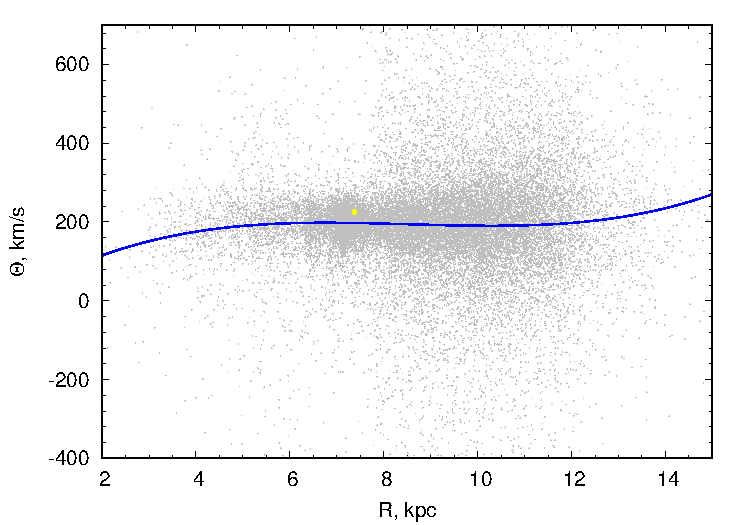
\includegraphics[width=1\linewidth]{pdf/rotc.pdf}
\end{minipage}
\end{figure}
\end{frame}

\begin{frame}{Заключение}
	\begin{itemize}
		\item Реализация алгоритма решения систем уравнений кинематической модели плоской подсистемы с исключением по избыточным невязкам в нескольких вариантах методом МНК.
		\item Исследование подсистемы звезд красного сгущения по данными каталога APOGEE-RC DR-14.
		\item Определение расстояния до центра Галактики, основных параметров движения Солнца в Галактике и параметров кинематической модели.
	\end{itemize}
\end{frame}


\begin{frame}{Ссылки}
 \begin{thebibliography}{10}
\beamertemplatebookbibitems
\bibitem{1} {\sc APOGEE-RC} {\em https://data.sdss.org/sas/dr13/apogee/vac/apogee-rc/cat/}
\bibitem{2} {\sc Bovy and etc.} {\em http://adsabs.harvard.edu/abs/2014arXiv1405.1032B}
\bibitem{3} {\sc Loktin A. V., Marsakov V. A. 2010} {Lectures on Stellar Astronomy, Rostov-na-Donu, pp. 282 (in Russian)}
\bibitem{3} {\sc Gromov A.O., Nikiforov I.I. 2016} {STÄCKEL-TYPE DYNAMIC MODEL OF THE GALAXY BASED
ON MASER KINEMATIC DATA}

\end{thebibliography}
\end{frame}

\begin{frame}{О каталоге}
	\begin{center}
	\begin{figure}[h]
\begin{minipage}[h]{0.8\linewidth}
\includegraphics[width=1\linewidth]{pdf/x_distr_dr13.pdf}
\end{minipage}
\end{figure}
	\end{center}
\end{frame}

\begin{frame}{О каталоге}
	\begin{center}
	\begin{figure}[h]
\begin{minipage}[h]{0.8\linewidth}
\includegraphics[width=1\linewidth]{pdf/y_distr_dr13.pdf}
\end{minipage}
\end{figure}
	\end{center}
\end{frame}

\begin{frame}{О каталоге}
	\begin{center}
	\begin{figure}[h]
\begin{minipage}[h]{0.8\linewidth}
\includegraphics[width=1\linewidth]{pdf/metals.pdf}
\end{minipage}
\end{figure}
	\end{center}
\end{frame}

\begin{frame}{О каталоге}
	\begin{center}
	\begin{figure}[h]
\begin{minipage}[h]{0.7\linewidth}
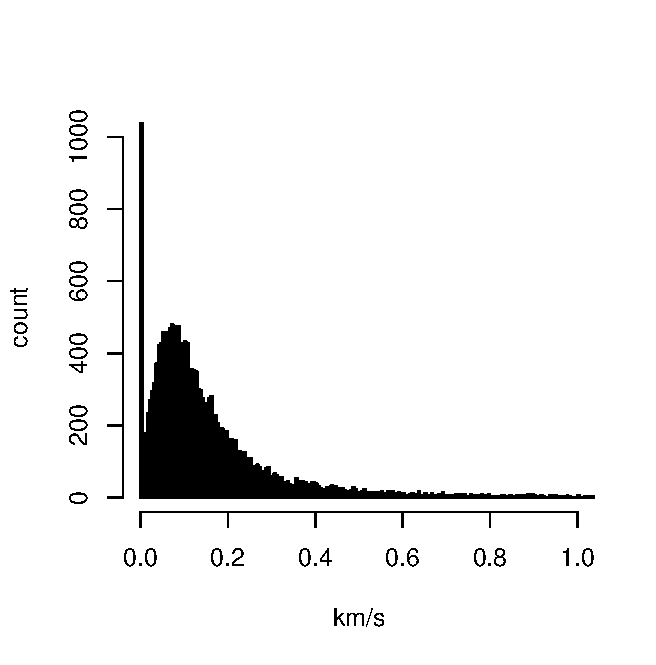
\includegraphics[width=1\linewidth]{pdf/vscatter.pdf}
\end{minipage}
\end{figure}
	\end{center}
\end{frame}

\begin{frame}{Стандартный вид профилей}
	\begin{center}
	\begin{figure}[h]
\begin{minipage}[h]{0.8\linewidth}
\includegraphics[width=1\linewidth]{pdf/profile_r0.pdf}
\end{minipage}
\end{figure}
	\end{center}
\end{frame}

\begin{frame}{Кинематически изолированные объекты}
	\begin{center}
	\begin{figure}[h]
\begin{minipage}[h]{0.8\linewidth}
\includegraphics[width=1\linewidth]{pdf/dr13/curre_4.pdf}
\end{minipage}
\end{figure}
	\end{center}
\end{frame}




\end{document}
